\chapter{One-Time-Pad}
Hier geht es um symmetrische Kryptosysteme.

\section{Caesar-Verfahren}
Sehr alt und bekannt. Kein Prinzip von Kerkchoff, sehr unsicher gegen Angreifer die das Verfahren kennen.

Aufgrund des kleinen Schlüsselraumes (26, effektiv 24) ist das Caesar Verfahren gegen Brute-Force schwach und aufgrund der Linearität auch gegen Wahrscheinlichkeitsanalyse schwach.

\section{Monoalphabetische Substitution}
Auf den ersten Blick scheint die Monoalphabetische Substitution eine Verbesserung des Caesar Verfahrens zu sein. Statt 26 Schlüssel gibt es 26! ($\approx$ 4 $\cdot$ $\text{10}^{\text{26}}$) Schlüssel. Jedoch, wenn man einen Teil des Klartextes erfährt, erkennt man welche Buchstaben ersetzt wurden.

Die Monoalphabetische Substitution gegen Brute-Force sehr gut geschützt, jedoch umso einfacher mit einer Häufigkeitsanalyse zu knacken.

\section{Vigenère Verfahren}
Bei allen monoalphabetischen Verfahren ist das Problem, dass ein Klartextzeichen immer durch dasselbe Chiffrezeichen ersetzt wird. Dies ist beim Vigenère Verfahren anders $\rightarrow$ polyalphabetisch. 
\begin{figure}[H]
	\centering
	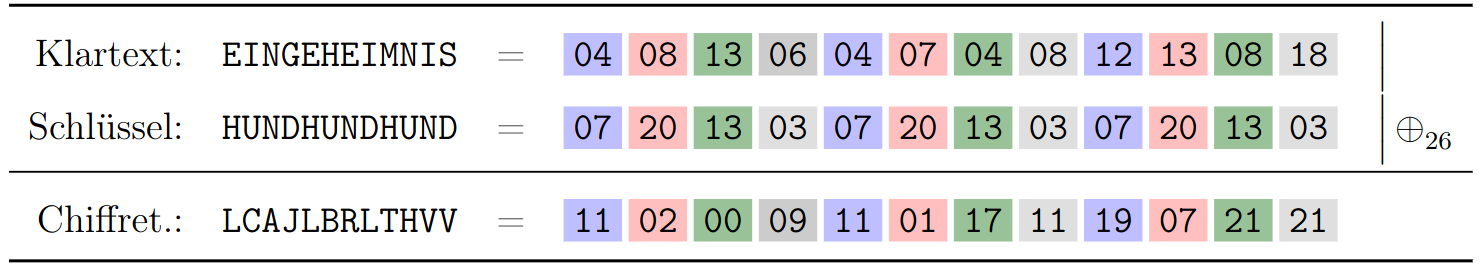
\includegraphics[width=1.0\linewidth]{figures/vigenere.png}
	\caption{Vigenère Verfahren}
\end{figure}
\textbf{Schachstelle:} Mit dem Kasiski Angriff lässt sich die Schlüsselwortlänge herausfinden, und mit einer Häufigkeitsanalyse dann das Schlüsselwort herausfinden.

\section{Vernam Verfahren}
Weiterentwicklung des Vigenère Verfahren. Anstatt ein Schlüsselwort zu wiederholen, wird ein Text eines leicht verfügbaren Buches (Telefonbuch, Bibel,...) verwendet. 

\section{One-Time-Pad}
Final Stufe: hier wird nun eine zufällige Kette als Schlüssel('wort') verwendet. Prinzipiell gutes Verfahren, jedoch: wirklich Zufällig Zeichenketten zu generieren ist schwer, weiters benötigt man bei einem $n$ langen Text, einen $n$ langen Schlüssel.
\textbf{Das One-Time-Pad ist in der Theorie sehr sicher, aber schwer in Praxis umzusetzen.}
